\chapter{Implementation of Non-dyson ADC}
In this chapter I describe the implementation of second order Non-dyson ADC of restricted Electron Affinity calculation in development version of \emph{adcman}.
\emph{Adcman} is a part of \emph{Q-Chem} package, which is a general-purpose electronic structure package based on C++ and Fortran.
It contains a variety of established and new methods implemented using innovative algorithms that enable fast calculations of large systems.
It's features include:
\begin{itemize}
	\item Variety of local, GGA, mGGA, hybrid, double-hybrid, dispersion-corrected, range separated functionals for DFT calculation.
	\item TDDFT and spin-flip-TDDFT
	\item Continuous Fast Multipole Method in HF and DFT
	\item Linear-scaling HF-exchange method
	\item Fourier transform Coulomb method
	\item Fast numerical integration of exchange-correlation with multiresolution exchange-correlation (mrXC)
	\item MP2
	\item SCS and SOS MP2
	\item CCD, QCISD, CCSD, OOCCD, VOOCCD
	\item EOM-XX-CCSD methods for open-shell and electronically excited species
	\item ADC methods
	\item CIS, TDDFT, CIS(D), and SOS-CIS(D) methods for excited states
\end{itemize}

\begin{figure}[h]
	\centering
	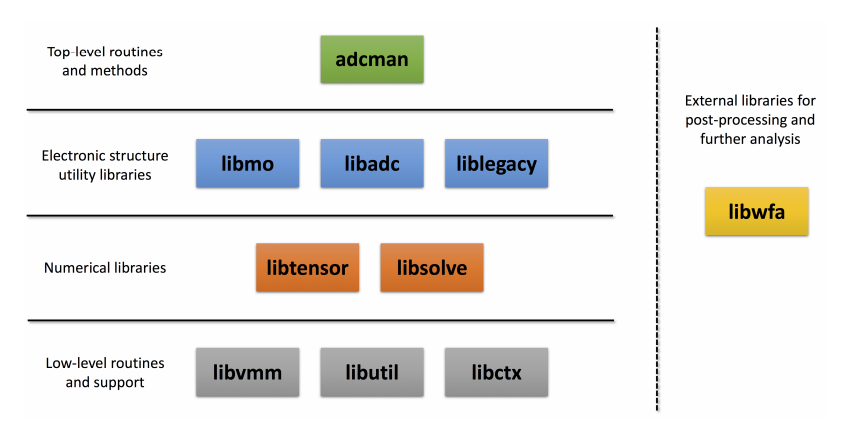
\includegraphics[width=\textwidth]{./figures/adcman.png}
	\caption{Overview of implementation of ADC methods in \emph{Q-Chem}}
	\label{codestucture}
\end{figure}

Then I will explain the overall code structure and then focus on my implementation part.
Finally I will present the results calculated by my implementation and compare them with CCSD.

\section{Code Overview and Structure}
The overview of implementation of ADC methods is in Fig. \ref{codestucture}.
All modules are written in the object-oriented C++ programming language. 
The adcman module contains all top-level routines and methods necessary for an ADC calculation. 
It coordinates the calculation process, sets up the solver and writes the results into an output file.
I implemented restricted calculation of EA part in adcman.

The next sub-level contains electronic structure related libraries and utilities.
\emph{liblegacy} is the gateway between the ADC code and the Q-Chem interface.
These routines help to import data from other Q-Chem modules, for example all SCF results and MOs, which are needed for the ADC calculation.
The \emph{libmo} module contains routines to set up the MO spaces, integrals and symmetry using the information imported from Q-Chem via the \emph{liblegacy} interface.
Hence, both \emph{libmo} and \emph{liblegacy} are important for ADC calculations, because all integrals and Fock-matrix elements are indexed and created corresponding to the additional restriction of the core space.
In the \emph{libadc} module, all ADC equations are implemented explicitly.
I also implemented restricted calculation of EA part in \emph{libadc}.

Furthermore, \emph{libmo} transforms the imported data in a format being compatible to the \emph{libtensor} \cite{libtensor} interface, which can be called the heart of the albegraic computation, since it contains all numerical routines to perform tensor algebra, which is the most time-consuming part all most of the quantum chemistry calculations.
\emph{libtensor} is specially designed for Post-Hartree-Fock electronic structure methods by including consideration of symmetries in the tensor structure.
These symmetries include Abelian point group symmetry, spin symmetry and other inner symmetry like that of two-electron integrals.
\begin{equation}
	\langle i j\| a b\rangle=-\langle j i\| a b\rangle=-\langle i j \| b a\rangle=\langle j i\| b a\rangle
\end{equation}
Thus, tensors of arbitrary order and size are stored in a blockwise manner to different kinds of symmetry to limit the amount of required memory and decrease the time needed.
The tensor operations in \emph{libtensor} are fully parallelized and efficiently implemented.

The second important numerical library is \emph{libsolve}, which contains all routines of
generic solvers, e.g the Davidson algorithm, which are called from the top-level adcman
routines. \emph{libsolve} is also based on the \emph{libtensor} interface. At last, there are low-level
routines, which are responsible for support and operations in the background. The libvmm
routines manage the virtual memory, while \emph{libctx} is a context manager based on key-value
mapping of data objects. All imported or generated objects, e.g. integrals, keywords,
tensors, vectors, etc., are stored in the context and can be easily accessed by other routines.
The libutil library contains further low-level machine-dependent routines.

The procedure of ADC calculation states as follows:
\begin{enumerate}
	\item A HF calculation is performed, and all information including one-electron integrals, two-electron integrals, MOs, eigenvalues, Overlap matrix, Fock matrix and point group symmetry are imported through \emph{libledacy} interface.
	\item All tensors calculated in the previous step are transformed from atomic orbital (AO) basis to MO basis by \emph{libmo} module.
	\item MP2 calculation is performed and results are printed.
	\item ADC secular matrix is constructed from the tensors in MO basis.
	\item Guess vectors which are required by Davidson algorithm are set up with correct symmetry.
	\item Davidson solver is started.
	\item When convergence requirements are met, ADC energies and transition amplitudes are printed.
	\item Other information required by adcman are printed.
\end{enumerate}

\section{Implementation of Non-dyson ADC}

\subsection{Implementation of ADC Secular Matrix}

We have illustrated the \emph{libtensor} library which can efficiently and conveniently realize tensor algebra.
From Eq \ref{KCeigen}, our final purpose is to calculate the eigenvalues and eigenvectors of ADC secular matrix.
However, usually we do not ask for all the eigenvalues and eigenvectors.
Instead, people are only interested in the few states with lowest energies.
Thus, full diagonalization will waste much effort on eigenstates that we are not interested in.
To solve this problem, we can use Davidson algorithm, which can determine eigenstates one by one with lower algorithmic complexity.
Since Davidson algorithm works by performing matrix vector product rather than direct access to matrix elements, we can rewrite the ADC secular matrix to matrix vector product form, i.e. calculate the result $W$ of matrix vector product when a vector $Y$ is given.

Before writing down the ADC secular matrix, we introduce some symbols:
\begin{equation}
	\begin{aligned}
		\langle pq \| rs \rangle&=V_{pq[rs]}
		\\
		\mathrm{t}_{\text { ijab }}&=\frac{\langle i j\| a b\rangle}{\varepsilon_{a}+\varepsilon_{\mathrm{b}}-\varepsilon_{i}-\varepsilon_{j}}
	\end{aligned}
\end{equation}

Up to second order, ADC secular matrix of ionization potential calculation is
\begin{equation}
	\mathrm{W}_{i}=\sum_{j} \mathrm{I}_{i j}^{(1)} \mathrm{Y}_{j}-\frac{1}{\sqrt{2}} \sum_{j k b}\langle j k\| b i\rangle Y_{j k b}
\end{equation}
for 1h part, where
\begin{equation}
\mathrm{I}_{i j}^{(1)}=-f_{i j}+\frac{1}{4}\left(1+\hat{\mathrm{P}}_{i j}\right) \sum_{a b k} t_{i k a b}\langle j k \| a b\rangle
\end{equation}
and
\begin{equation}
	\mathrm{W}_{i j a}=\sum_{\mathrm{b}} f_{a b} Y_{i j b}-\left(1-\hat{\mathrm{P}}_{i j}\right) \sum_{k} f_{i k} \mathrm{Y}_{k j a}+\frac{1}{\sqrt{2}} \sum_{k}\langle i j\| k a\rangle \mathrm{Y}_{k}
\end{equation}
for 1p-2h part.

Up to second order, ADC secular matrix of EA calculation is
\begin{equation}
	\mathrm{W}_{a}=\sum_{b} \mathrm{I}_{a b}^{(1)} \mathrm{Y}_{b}+\frac{1}{\sqrt{2}} \sum_{b c j}\langle b c\| j a\rangle Y_{b c j}
\end{equation}
for 1p part, where
\begin{equation}
\mathrm{I}_{a b}^{(1)}=-f_{a b}-\frac{1}{4}\left(1+\hat{\mathrm{P}}_{a b}\right) \sum_{i j c} t_{i j a c}\langle b c \| i j\rangle
\end{equation}
and
\begin{equation}
	\mathrm{W}_{a b i}=\sum_{\mathrm{b}} f_{i j} Y_{a b j}-\left(1-\hat{\mathrm{P}}_{a b}\right) \sum_{c} f_{a c} \mathrm{Y}_{c b i}-\frac{1}{\sqrt{2}} \sum_{c}\langle a b\| c i\rangle \mathrm{Y}_{c}
\end{equation}
for 1h-2p part.

The implementation of ADC secular matrix is by a class \emph{adc2\_matrix}:

\lstinputlisting[language=C++]{./code/adc2matrix.h}

\subsection{Implementation of Setting up Guess Vectors}

Before the Davidson algorithm starts, guess vectors need to be set up for the first matrix vector product.
Usually, the setting up of guess vectors should be subjected to some principles: computationally cheap and close to the final eigenvectors.
A simple idea is to use eigenvectors of some simple approximation of the ADC secular matrix.
In the implementation in Q-Chem, the approximation of second order ADC secular matrix is chosen to be the diagonal elements.
Since people usually care about the states with lowest enegies, the guess vectors should be chosen to be those with smallest diagonal elements.
Mathmatically, if $d_a=K_{aa}+C_{aa}$, and the $n$ smallest elements are $d_{k_1}<d_{k_2}< \dots <d_{k_n}$, then the $m$th guess vector should be 
\begin{equation}
	v^m_p=\delta_{p, k_m}
\end{equation}

Of course, we will get correct results if we set up guess vectors in the above way.
However, since Hamiltonian is commutable with total spin operator $S^2$, it is often required the diagonalization of Hamiltonian also diagonalizes $S^2$.
Thus, it is required that the initial guess vectors should have correct spin symmetry.
In addition, the 1h-2p guess vectors themselves has permutation symmetry
\begin{equation}
	V_{abi}=-V_{bai}
\end{equation}
, which is easy to deal with. Thus we will focus on spin symmetry of guess vectors.

For restricted calculation, electrons in ground state are always paired, thus the EA does not depend on whether alpha or beta electron is added, thus we can always choose it to be alpha electron.
Thus, the final state will be restricted to $m_s=\frac{1}{2}$.

For 1p guess vectors, there is no choice for spin since the added electron must be spin spin, and thus
\begin{equation}
	v^m_{a s}=\delta_{a, k_m} \delta_{s, \alpha}
\end{equation}
where $s$ is the spin of orbital a.

For 1h-2p guess vectors, there are two options:
\begin{itemize}
	\item One particle is alpha, one particle is beta, and the hole is beta.
	\item All two particles and the hole are alpha.
\end{itemize}

Thus there are totally three configurations (two for the first case and one for the second case).
To correcctly set up spin symmetry of guess vectors, we need to form linear combinations of these three configurations that are diagonal under $S^2$.
In fact, the coefficients of the linear combinations are refered as Clebsch-Gordan coefficients.
By refering to table of Clebsch-Gordan coefficients, the three final spin states reads:
\begin{equation}
	\begin{array}{|l|l|}
		\hline
		S=\frac{1}{2} & \sqrt{\frac{1}{2}} \ket{\alpha_p \beta_p \beta_h} - \sqrt{\frac{1}{2}} \ket{\beta_p \alpha_p \beta_h}
		\\
		\hline
		S=\frac{1}{2} & \sqrt{\frac{2}{3}} \ket{\alpha_p \alpha_p \alpha_h} - \sqrt{\frac{1}{6}} \ket{\alpha_p \beta_p \beta_h} - \sqrt{\frac{1}{6}} \ket{\beta_p \alpha_p \beta_h}
		\\
		\hline
		S=\frac{3}{2} & \sqrt{\frac{1}{3}} \ket{\alpha_p \alpha_p \alpha_h} + \sqrt{\frac{1}{3}} \ket{\alpha_p \beta_p \beta_h} + \sqrt{\frac{1}{3}} \ket{\beta_p \alpha_p \beta_h}
		\\
		\hline
	\end{array}
\end{equation}

The above tables works when the spacial orbital of two particles are different, otherwise they must have different spins, which means the second case is not allowed.
In such situation, the two paricles are paired, and will not contribute to the total spin.
Thus it reduces to the 1p case.

To summarize, if $a \neq b$, the first guess vector for spin $\frac{1}{2}$ is
\begin{equation}
	\begin{array}{ll}
		V_{a \alpha, b \beta, i \beta}=\frac{1}{2} & V_{b \beta, a \alpha, i \beta}=-\frac{1}{2} 
		\\
		V_{a \beta, b \alpha, i \beta}=-\frac{1}{2} & V_{b \alpha, a \beta, i \beta}=\frac{1}{2} 
	\end{array}
\end{equation}
the second guess vector for spin $\frac{1}{2}$ is 
\begin{equation}
	\begin{array}{ll}
		V_{a \alpha, b \alpha, i \alpha}=\sqrt{\frac{1}{3}} & V_{b \alpha, a \alpha, i \beta}=-\sqrt{\frac{1}{3}} 
		\\
		V_{a \alpha, b \beta, i \beta}=-\sqrt{\frac{1}{12}} & V_{b \beta, a \alpha, i \beta}=\sqrt{\frac{1}{12}} 
		\\
		V_{a \beta, b \alpha, i \beta}=-\sqrt{\frac{1}{12}} & V_{b \alpha, a \beta, i \beta}=\sqrt{\frac{1}{12}} 
	\end{array}
\end{equation}
the guess vector for spin $\frac{3}{2}$ is
\begin{equation}
	\begin{array}{ll}
		V_{a \alpha, b \alpha, i \alpha}=\sqrt{\frac{1}{6}} & V_{b \alpha, a \alpha, i \beta}=-\sqrt{\frac{1}{6}} 
		\\
		V_{a \alpha, b \beta, i \beta}=\sqrt{\frac{1}{6}} & V_{b \beta, a \alpha, i \beta}=-\sqrt{\frac{1}{6}} 
		\\
		V_{a \beta, b \alpha, i \beta}=\sqrt{\frac{1}{6}} & V_{b \alpha, a \beta, i \beta}=-\sqrt{\frac{1}{6}} 
	\end{array}
\end{equation}
if $a=b$, the first guess vector for spin $\frac{1}{2}$ is
\begin{equation}
	\begin{array}{ll}
		V_{a \alpha, b \beta, i \beta}=\frac{1}{2} & V_{b \beta, a \alpha, i \beta}=-\frac{1}{2} 
		\\
		V_{a \beta, b \alpha, i \beta}=-\frac{1}{2} & V_{b \alpha, a \beta, i \beta}=\frac{1}{2} 
	\end{array}
\end{equation}
the second guess vector for spin $\frac{1}{2}$ is 
\begin{equation}
	\begin{array}{ll}
		V_{a \alpha, b \beta, i \beta}=\frac{1}{2} & V_{b \beta, a \alpha, i \beta}=\frac{1}{2} 
		\\
		V_{a \beta, b \alpha, i \beta}=\frac{1}{2} & V_{b \alpha, a \beta, i \beta}=\frac{1}{2} 
	\end{array}
\end{equation}

For unrestricted case, it is much more complicated.
Although I do not implement it, it does not hurt to discuss a little about this.

Consider the ground state of a system with $p$ net positive charge, in which $p_{\alpha}$ are spin alpha while $p_{\beta}$ are spin beta.
After affinity of an electron, which could be either spin alpha or spin beta.
Thus, the general question is the linear combination of $n_{\alpha}$ alpha spins and $n_{\beta}$ beta spins, where
\begin{equation}
	\begin{array}{lll}
		n_{\alpha}=p_{\alpha} + 1, & n_{\beta}=p_{\beta} & \text{if added alpha electron}
		\\
		n_{\alpha}=p_{\alpha}, & n_{\beta}=p_{\beta} + 1 & \text{if added beta electron}
	\end{array}
\end{equation}

The $n=n_{\alpha} + n_{\beta}$ electrons will genrate $2^n$ configurations.
However, Clebsch-Gordan coefficients only works for addition of two spins.
Thus, an recursive approach is needed to deal with the $n$ spin case.

\section{Results of Calculation}

In this section, I will present a benchmark calculation of the EA-ADC(2) method.
The calculated results are compared with HF, DFT with B3LYP functional and CCSD.
CCSD is used for comparison because CCSD is a widely used Post-Hartree-Fock method to include consideration of electron correlation, which is very reliable.
HF and DFT are used for comparison to show that ADC can perform better than these low-level results, otherwise we don't need these high-level methods, which are computationally more expensive.
For this benchmark calculation, small moleculars 
$\text{H}_2\text{O}$, $\text{NH}_3$, $\text{CO}_2$, $\text{LiH}$,
$\text{LiF}$, $\text{N}_2\text{O}$, $\text{CH}_4$,
$\text{C}_2\text{H}_6$, $\text{CH}_2\text{O}$, $\text{HCN}$ are chosen, and the basis set is chosen to be 6-31g.
The results of HF and DFT are obtained by subjecting the ground state energy of original molecule and anion with -1 charge.
Since both HF and DFT are size consistent, it will not cause problem of size consistency.

\begin{table}
	\centering
	\caption{first EA of small molecules under cc-pVTZ basis}
	\label{firstEA}
\begin{tabular}{|c|c|c|c|c|}
	\hline
	Molecules              & HF    & B3LYP & ADC(2) & CCSD  \\ \hline
	$\text{CO}_2$          & -4.64 & -3.46 & -3.47  & -3.73 \\ \hline
	LiF                    & 0.14  & 0.29  & 0.18   & 0.17  \\ \hline
	LiH                    & 0.08  & 0.25  & 0.12   & 0.13  \\ \hline
	$\text{N}_2\text{O}$   & -2.95 & -2.8  & -2.8   & -3.22 \\ \hline
	$\text{H}_2\text{O}$   & -3.72 & -2.93 & -3.27  & -3.31 \\ \hline
	$\text{NH}_3$          & -3.62 & -2.78 & -3.08  & -3.13 \\ \hline
	$\text{CH}_4$          & -3.82 & -2.96 & -3.27  & -3.31 \\ \hline
	$\text{C}_2\text{H}_2$ & -4.17 & -2.93 & -3.33  & -3.5  \\ \hline
	HCN                    & -3.71 & -2.99 & -3.09  & -3.29 \\ \hline
	$\text{CH}_2\text{O}$  & -2.15 & -1.47 & -1.62  & -1.92 \\ \hline
\end{tabular}
\end{table}
\begin{figure}[ht]
	\centering
	\begin{subfigure}[b]{0.42\linewidth}
		\centering
		\includegraphics[width=\linewidth]{./figures/higher/C2H2.pdf}
	\end{subfigure}
	\begin{subfigure}[b]{0.42\linewidth}
		\centering
		\includegraphics[width=\linewidth]{./figures/higher/CH2O.pdf}
	\end{subfigure}
	\begin{subfigure}[b]{0.42\linewidth}
		\centering
		\includegraphics[width=\linewidth]{./figures/higher/CH4.pdf}
	\end{subfigure}
	\begin{subfigure}[b]{0.42\linewidth}
		\centering
		\includegraphics[width=\linewidth]{./figures/higher/CO2.pdf}
	\end{subfigure}
	\begin{subfigure}[b]{0.42\linewidth}
		\centering
		\includegraphics[width=\linewidth]{./figures/higher/H2O.pdf}
	\end{subfigure}
	\begin{subfigure}[b]{0.42\linewidth}
		\centering
		\includegraphics[width=\linewidth]{./figures/higher/HCN.pdf}
	\end{subfigure}
	\begin{subfigure}[b]{0.42\linewidth}
		\centering
		\includegraphics[width=\linewidth]{./figures/higher/LiF.pdf}
	\end{subfigure}
	\begin{subfigure}[b]{0.42\linewidth}
		\centering
		\includegraphics[width=\linewidth]{./figures/higher/LiH.pdf}
	\end{subfigure}
	\begin{subfigure}[b]{0.42\linewidth}
		\centering
		\includegraphics[width=\linewidth]{./figures/higher/N2O.pdf}
	\end{subfigure}
	\begin{subfigure}[b]{0.42\linewidth}
		\centering
		\includegraphics[width=\linewidth]{./figures/higher/NH3.pdf}
	\end{subfigure}
	\caption{First 10 EAs calculated by ADC(2) and CCSD on small molecules}
	\label{higher}
\end{figure}
On the other hand, choice of appropriate basis is very important for EA calculation.
The reason is that anions bind their outermost electrons rather weakly, and hence their valence-range electron densities are diffuse, which means that the use of diffuse functions is an important requirement for basis in EA calculation, and also means that a large basis space is needed to achieve accurate results. One of the basis that satisfying this requirement is cc-pVXZ basis (X=D/T/Q/5 \dots). \cite{newpaper}

We first calculate the first EA energy for these molecules.
In this calculation, cc-pVTZ basis and CCSD are used for an accurate geometry optimization and then cc-PVTZ basis is used for EA calculation.
The results are shown in Table \ref{firstEA}

We can see from the results that ADC(2) matches well with CCSD (mean derivation is 0.15 eV), while both HF and DFT give great derivation (mean derivations are 0.34 eV for HF and 0.39 eV for DFT).
We can also find that HF tends to underestimate EA, and DFT tends to overestimate EA.

Then we compare higher order electron affinities calculated by ADC(2) and CCSD on these small molecules.
Results are shown in Fig. \ref{higher}
As is shown in the figure, ADC(2) results match well with CCSD for the first few EAs among all the molecules.
However, they give large errors for higher orders of EAs, and ADC almost always gives lower EAs for these states.
We can also find that generally, disagreements comes later for large molecules (CO$_2$, N$_2$O and C$_2$H$_2$).

If we look into the amplitudes of 1p and 1h-2p parts, we can find that when a state is dominated by 1p part, ADC(2) and CCSD usually give similar results; however,when it is dominated by 1h-2p part, two theories disagree with a large probability.
This means that the ADC(2) give good results for 1p part but bad result for 1h-2p part, and it usually overestimate the energies for 1h-2p part.
Then we will analyze the reason for this.
Eq \ref{generalTEO} in ISR theory tells us that in the case of ADC(2), TEO of 1p part is second order, while TEO of 1h-2p part is zeroth order.
Thus, ADC(2) gives larger error for 1h-2p results while describes 1p part accurately, compared with CCSD.

On the other hand, we can see from the structure of ADC(2) secular matrix \ref{ADC2} that only $K_2$ is included for 1h2p-1h2p part, thus there is no mix between 1h2p states, which can not effectively decrease energies.
This problem will be solved in ADC(3), since $C^1_{11}$ is also included in 1h2p-1h2p part, and thus TEO for 1h2p states is second order, which is much better.

Another problem for these results is that first EAs of all molecules except Li$_H$ and Li$_F$ are negative, which means that such states are not stable and the anions will automatically decompose into a neutral and a free electron, which is totally unphysical.

This problem comes from two parts.
The first part is finite basis, and the second part is incorrect result of electron correlation.
The first part can principly be solved by complete basis set (CBS).
One famous CBS is cc-pVXZ basis \cite{CBS}, which should give asymptotic results when $X \rightarrow \infty$.
Then we perform calculations for LiH, LiF, CO$_2$ and N$_2$O under these basis.
The results are shown in Table \ref{ccpVXZ}.
\begin{table}
	\centering
	\caption{first EA calculated by ADC(2) and CCSD for cc-pVDZ, cc-pVTZ cc-pVDZ}
	\label{ccpVXZ}
	\begin{tabular}{|c|c|c|c|c|c|c|}
		\hline
		\multirow{2}{*}{Molecules} & \multicolumn{3}{c|}{ADC(2)} & \multicolumn{3}{c|}{CCSD}   \\ \cline{2-7} 
								   & cc-pVDZ & cc-pVTZ & cc-pVQZ & cc-pVDZ & cc-pVTZ & cc-pVQZ \\ \hline
		LiH                        & 0.06    & 0.12    & 0.20    & 0.07    & 0.13    & 0.20    \\ \hline
		LiF                        & 0.12    & 0.18    & 0.26    & 0.11    & 0.17    & 0.25    \\ \hline
		CO$_2$                     & -4.97   & -3.47   & -2.52   & -5.21   & -3.73   & -2.73   \\ \hline
		N$_2$O                     & -3.55   & -2.80   & -2.48   & -3.92   & -3.22   & -2.92   \\ \hline
	\end{tabular}
\end{table}
As we can see in the results, the first EA increases when $X$ increases among all of the molecules, which means basis set plays a very imporant role to get positive EAs.
However, cc-pVXZ is a really large basis set, thus a cc-pV5Z is difficult for these molecules and is not given in this benchmark calculation.

For the second part of the reason, which is incorrect electron correlation, it still remains unsolved until now and is one of the center problems of electronic structure.
Many methods are also under development to solve this problem.
Thus, it is not surprising to see that both ADC(2) and CCSD sometimes give bad results.
